\documentclass[a4paper]{article}

\usepackage[english]{babel}
\usepackage[utf8]{inputenc}
\usepackage{amsmath}
\usepackage{graphicx}
\usepackage[colorinlistoftodos]{todonotes}
\usepackage{titling}
\usepackage{listings}
\usepackage[T1]{fontenc}
\usepackage{array,multirow,makecell}
\setcellgapes{1pt}
\makegapedcells
\newcolumntype{R}[1]{>{\raggedleft\arraybackslash }b{#1}}
\newcolumntype{L}[1]{>{\raggedright\arraybackslash }b{#1}}
\newcolumntype{C}[1]{>{\centering\arraybackslash }b{#1}}

\newcommand{\subtitle}[1]{%
  \posttitle{%
    \par\end{center}
    \begin{center}\large#1\end{center}
    \vskip0.5em}%
}
\lstset{%
  basicstyle=\scriptsize\sffamily,%
  commentstyle=\footnotesize\ttfamily,%
  frameround=trBL,
  frame=single,
  breaklines=true,
  showstringspaces=false,
  numbers=left,
  numberstyle=\tiny,
  numbersep=10pt,
  keywordstyle=\bf
}





%%%%%%%%%%%%%%%%%%%%%%%%%%%%%%%%%%%%%%%%%%%%%%%%%%%%
% Raport Headers:
%%%%%%%%%%%%%%%%%%%%%%%%%%%%%%%%%%%%%%%%%%%%%%%%%%%%
\title{Image and signal processing: Additional Computer exercise 3\\CE03G02T05}
\author{PASHEVICH Alexander, SID-LAKHDAR Riyane}
\date{15/11/2015}

\begin{document}


\maketitle

\section{Definition of the problem}
When the human eye looks at an image, it is much more sensitive to the variation of colors than to the colors itself.   The notion of color variation is what we call "contrast".\\
\textbf{[Add the the same image before and after stretching]}\\

The problem is that, due to devices problem, pictures may have a lot of different colors which are transcribed in a very narrow gap of gray colors.   This way, human eyes can't make the difference between this different colors.\\
            \begin{figure}[!htb]\centering
                \begin{minipage}{0.45\textwidth} \frame{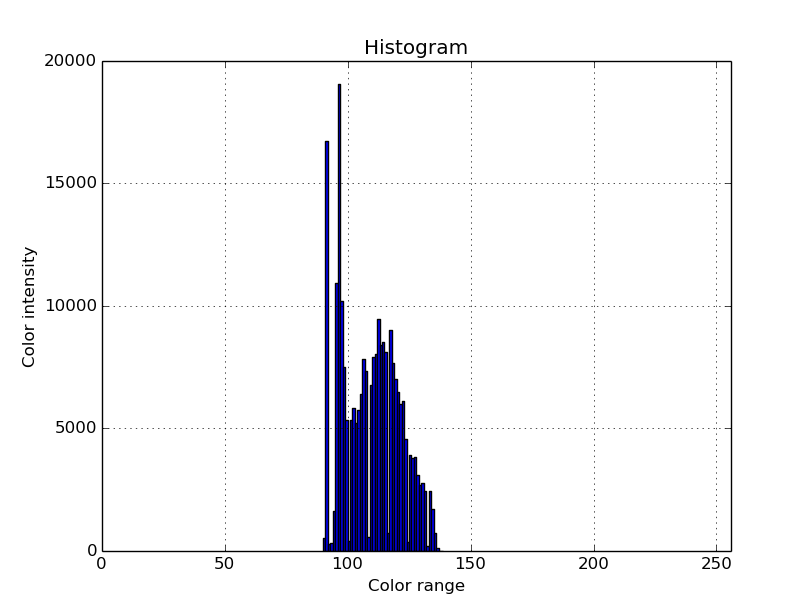
\includegraphics[width=\linewidth]{histogram_of_contrasted_picture.png}} \end{minipage}
                \caption{Histogram of not contrasted picture}
			\end{figure}

In this exercise, we will present to you a technique to fix the contrast problem: "Contrast Stretching ".



\section{Explaining the formula}
	\begin{equation*}
	\begin{aligned}
	y[n] &= (x[n] - actualMin) *\frac{newMax - newMin}{currentMax - currentMin} + newMin\\
    y[n] &= (x[n] - actualMin) * \alpha + newMin
	\end{aligned}
	\end{equation*}
    
    \begin{itemize}
		\item This function is strictly increasing as $\alpha > 0$
        \item Its minimal value is 
        	\begin{equation*}
			\begin{aligned}
				y_{min}[n] &= \alpha (x_{min}[n] - currentMin) + newMin \\
				y_{min}[n] &= \alpha (currentMin - currentMin) + newMin \\
				y_{min}[n] &= newMin
			\end{aligned}
			\end{equation*}
        \item Its maximal value is
        	\begin{equation*}
			\begin{aligned}
				y_{min}[n] &= \frac{newMax - newMin}{currentMax - currentMin} * (x_{max}[n] - currentMin) + newMin\\
				y_{min}[n] &= \frac{newMax - newMin}{currentMax - currentMin} * (currentMax - currentMin) + newMin\\
				y_{min}[n] &= newMax - newMin + newMin\\
				y_{min}[n] &= newMax
            \end{aligned}
            \end{equation*}
	\end{itemize}




\section{How to use this formula to solve our problem}
	The aim of this function is to take a set of values ranked in the gap [currentMin, currentMax] and to spread them on the bigger gap [newMin, newMax].\\

    This function is also linear (with a positive slope $\alpha$).  Thus the distance between the new ranks of colors will stay constant.
    
    \begin{figure}[ht!]
    \lstset{language=Python}
    \begin{lstlisting}
def stretchContrast(inputImage, newRangeMin, newRangeMax):
    actualMax = myMax(img.flatten())
    actualMin = myMin(img.flatten())
    outputImage = np.zeros(len(inputImage))
    for i in range(len(inputImage)):
        newVal = newRangeMin + (newRangeMax - newRangeMin) / (actualMax - actualMin) * (inputImage[i] - actualMin)
        outputImage[i] = newVal
    return outputImage

    \end{lstlisting}
    \caption{Python code to apply the stretch contrast method on an image.}
    \label{stretchContrast.py}
	\end{figure}


\section{Experimental results}
            \begin{figure}[!htb]\centering
                \begin{minipage}{0.45\textwidth} \frame{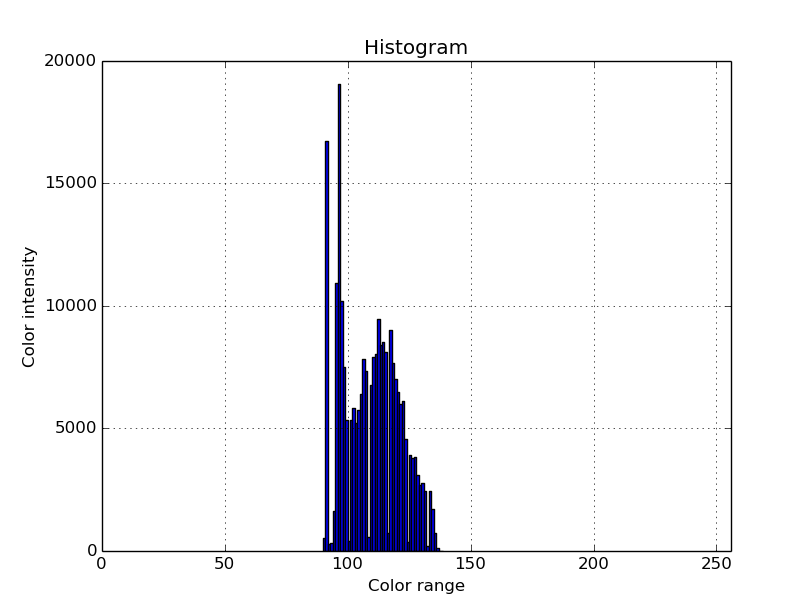
\includegraphics[width=\linewidth]{histogram_of_contrasted_picture.png}} \end{minipage}
                \begin{minipage}{0.45\textwidth} \frame{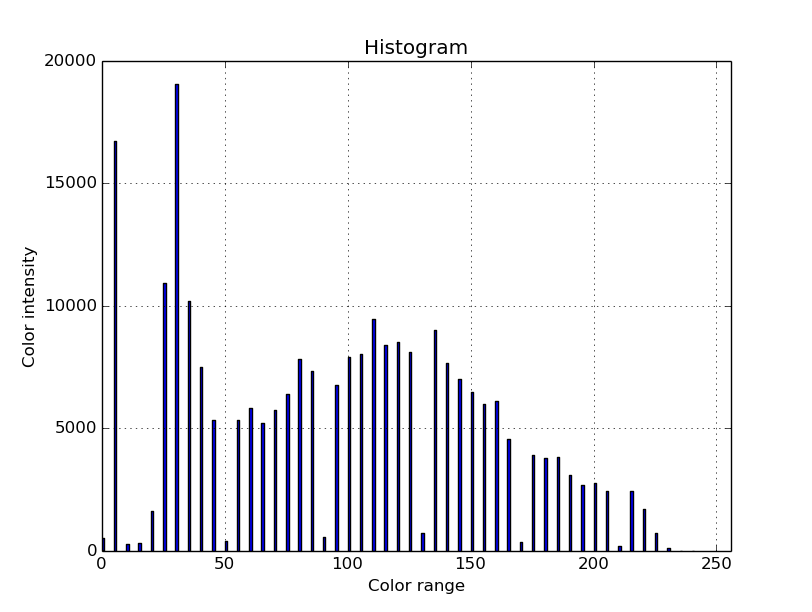
\includegraphics[width=\linewidth]{histogram_of_stretched_picture.png}} \end{minipage}
                \begin{minipage}{0.45\textwidth} \frame{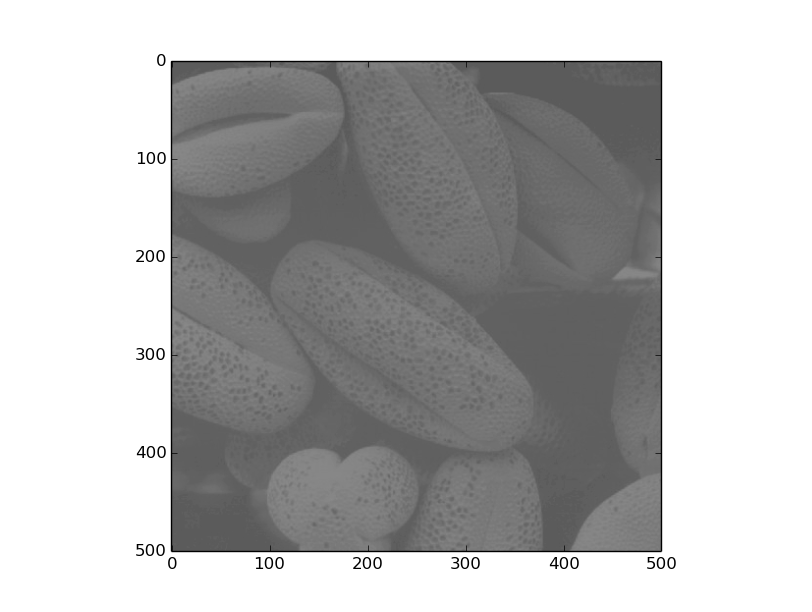
\includegraphics[width=\linewidth]{contrasted_picture.png}} \end{minipage}
                \begin{minipage}{0.45\textwidth} \frame{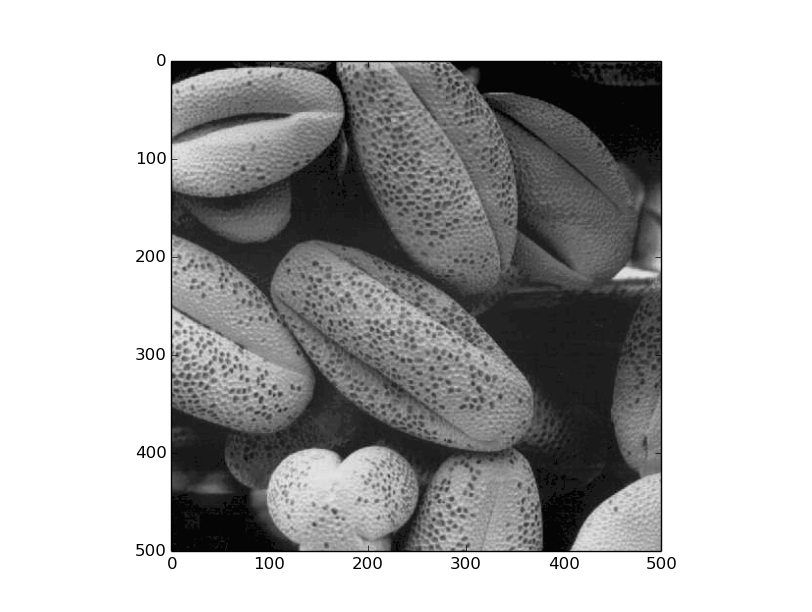
\includegraphics[width=\linewidth]{stretched_picture.png}} \end{minipage}
                \caption{Histogram and corresponding pictures before and after applying the contrast stretching}
                \label{experimentalResult.png}
			\end{figure}

	Let consider the picture Figure (fig \ref{experimentalResult.png}).   We can notice on the grey color histogram of this picture that the most used colors are in a small gap of colors: [90, 140].   An the other gaps are unused: [0, 90] and [140, 255].\\

    Thanks to our previous algorithm, we have been able to map each color from the initial image to a new color.  As we can see on the right histogram, this set of colors is much more expanded.   Thus, the created image is much more clear for the human eyes as we have expanded the difference between the used colors.

\section{Advantages of the "Contrast Stretching method" }
	The advantage of this technique is obviously its ease of implementation.   We have shown as well that our algorithm has a very interesting complexity: for a picture of n pixels, the complexity of our algorithm is c(n) = O(2n).  (O(n) to build the histogram and compute the min and max values, plus O(n) to build the output picture's pixels).\\

In an other hand, we can notice that our algorithm may be applied no matter what is the encoding used for a pixel:  In our example, we have used the PGM format, which means that each pixel is encoded on 8 bits.   Thus the max value in our formula is $2^{8} -1 = 255$.  But this method may be adapted to any kind of pixel encoding by simply adapting the max and min values in the formula to the max and min value of the used codes.


\section{Limits of the "Contrast Stretching method" }
\textbf{A faire : changer ce paragraph (copier coller wiki)}\\
The problem with this is that a single outlying pixel with either a very high or very low value can severely affect the value of c or d and this could lead to very unrepresentative scaling. Therefore a more robust approach is to first take a histogram of the image, and then select c and d at, say, the 5th and 95th percentile in the histogram (that is, 5\% of the pixel in the histogram will have values lower than c, and 5\% of the pixels will have values higher than d). This prevents outliers affecting the scaling so much. 
\end{document}


